\newif \ifshare
% \sharetrue % Comment this if you want animation
\ifshare % "Share mode" without animation.
\documentclass[table, trans, aspectratio = 169]{beamer}
\else % "Presentation mode" with animation.
\documentclass[table, aspectratio = 169]{beamer}
\fi
\usepackage[T1]{fontenc}
\usepackage{color}
\usepackage{graphicx}
\usepackage{subfig}
\usepackage{diagbox}
\usepackage{amssymb}% http://ctan.org/pkg/amssymb
\usepackage{pifont}% http://ctan.org/pkg/pifont
\newcommand{\cmark}{\ding{51}}%
\newcommand{\xmark}{\ding{55}}%

% \pdfsuppresswarningpagegroup=1

\let\pgfmathMod=\pgfmathmod\relax

\graphicspath{{../figs/PDF/}}

\usetheme{Boadilla}

\definecolor{struct}{HTML}{03a9f4}
\definecolor{alert}{HTML}{f44336}
\definecolor{example}{HTML}{aeea00}
\definecolor{good}{HTML}{8bc34a}
\definecolor{notgoodnotbad}{HTML}{ff9800}

\setbeamercolor{structure}{fg = struct}
\setbeamercolor{normal text}{fg = white, bg = black}
\setbeamercolor{example text}{fg = example}
\setbeamercolor{alerted text}{fg = alert}
\setbeamercolor{footline}{fg = white}

\title[Widsom Exchange]{Linux kernel development using QEMU}
\subtitle{Wisdom Exchange}
\author[Francis Laniel (\texttt{flaniel@linux.microsoft.com})]{Francis Laniel\\\texttt{flaniel@linux.microsoft.com}}
\date{6th September 2023}

% Custom title page.
\defbeamertemplate*{title page}{customized}[1][]{
	\centering
	\usebeamerfont{title}\usebeamercolor[fg]{title}\inserttitle\par
	\usebeamerfont{subtitle}\usebeamercolor[fg]{subtitle}\insertsubtitle\par
	\bigskip
	\usebeamerfont{author}\usebeamercolor[fg]{normal text}\textbf{\insertauthor}\par
	\bigskip
	\usebeamerfont{date}\usebeamercolor[fg]{normal text}\textbf{\insertdate}\par
	\bigskip
	\bigskip

	\begin{columns}
		\begin{column}{.5\textwidth}
			\centering

			\includegraphics[scale=2]{microsoft.pdf}
		\end{column}
		\begin{column}{.5\textwidth}
			\centering

			\includegraphics{kinvolk.pdf}
		\end{column}
	\end{columns}
}

\begin{document}
	% Put these parameters here to avoid compilation error:
	% "! LaTeX Error: Missing \begin{document}."
	% Remove the navigation bar, this is useless...
	\setbeamertemplate{navigation symbols}{}
	% Use square instead of bubbles, see:
	% https://tex.stackexchange.com/a/69721
	\setbeamertemplate{section in toc}[square]
	% Modify the shaded value to 60% instead of 20%, see:
	% https://tex.stackexchange.com/a/66703
	\setbeamertemplate{sections/subsections in toc shaded}[default][50]
	% Use circle instead of bubbles for itemize, see:
	% \setbeamertemplate{itemize items}[circle]
	\setbeamertemplate{itemize items}[square]
	\setbeamertemplate{enumerate items}[square]

	\maketitle

	\section{Introduction}
	\begin{frame}
		\frametitle{The Linux kernel}

		First released in 1991 \cite{torvalds_what_nodate}:
		\begin{quote}
			Hello everybody out there using minix -
			I'm doing a (free) operating system (just a hobby, won't be big and professional like gnu) for 386(486) AT clones.
		\end{quote}

		\onslide<2->{
			Nowadays, it has many subsystems and works on plenty of architecture \cite{shulyupin_linux_2018}:

			\begin{figure}
				\centering

				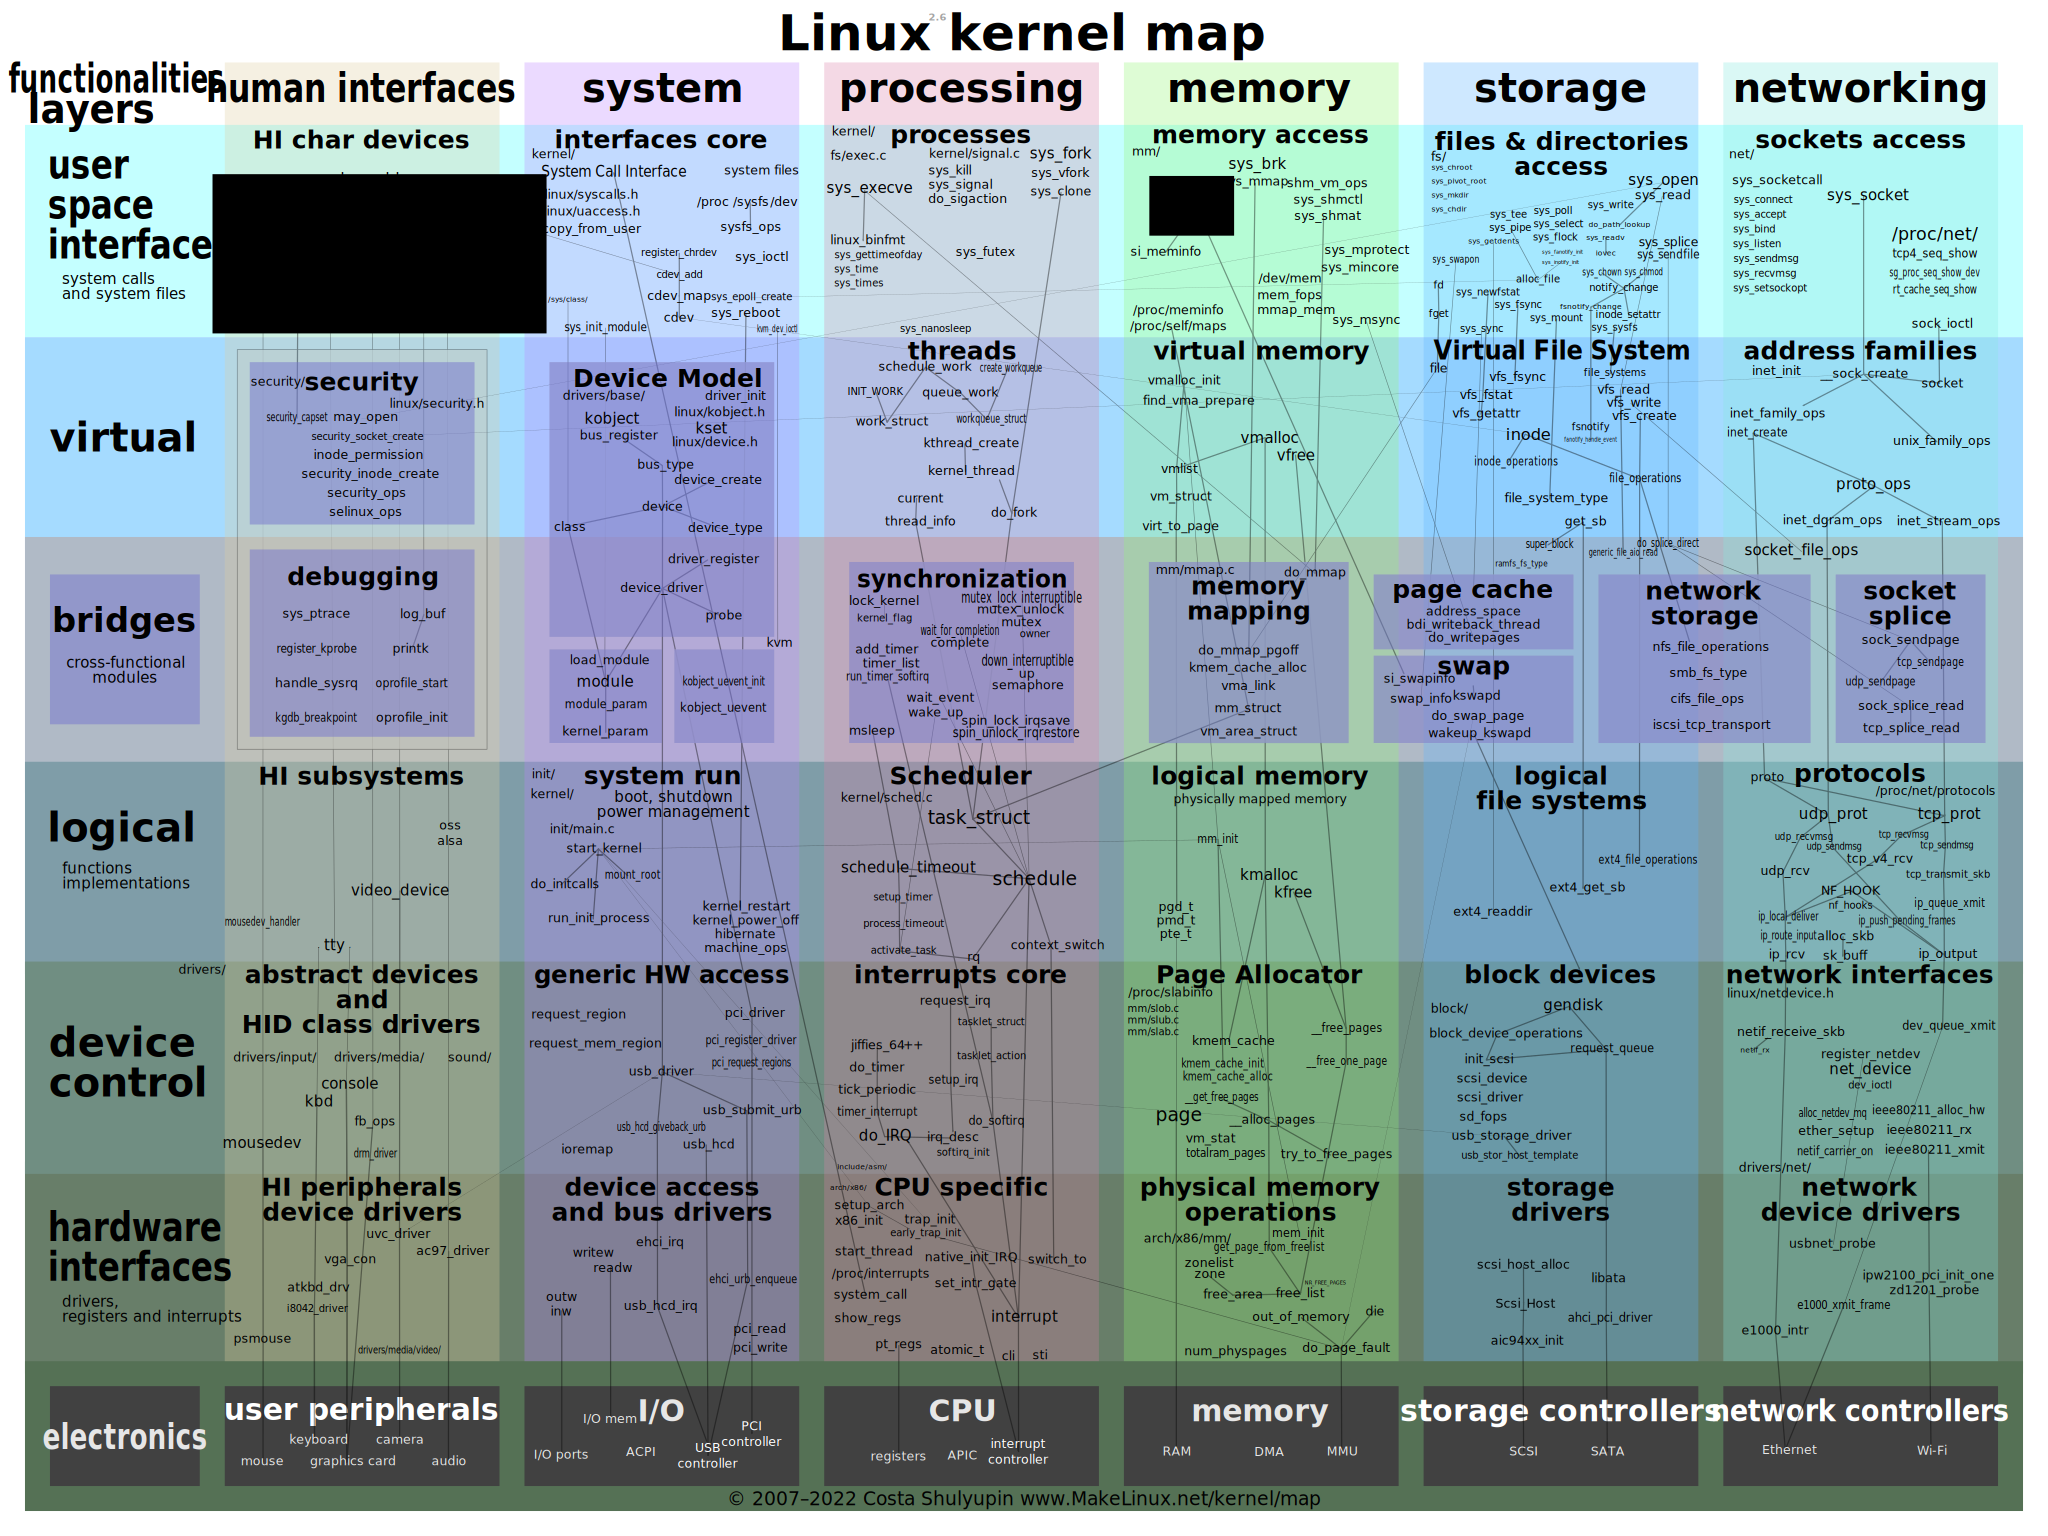
\includegraphics[scale=.1]{LKM.pdf}
			\end{figure}
		}
	\end{frame}

	\begin{frame}[fragile]
		\frametitle{Linux kernel development}
		\framesubtitle{The basics}

		\begin{verbatim}
			$ git clone git://git.kernel.org/pub/scm/linux/kernel/git/torvalds/linux.git
			$ cd linux
			$ make defconfig
			$ make -j$(nproc)
		\end{verbatim}
	\end{frame}

	\begin{frame}[fragile]
		\frametitle{Linux kernel development}
		\framesubtitle{Good to know}

		You do not have access to \texttt{libc}, but the kernel provides good API for:
		\begin{itemize}
			\item string manipulation with \texttt{string.h} (\textit{e.g.} \texttt{strcpy()}),
			\item (circular double-linked) list manipulation with \texttt{list.h} (\textit{e.g.} \texttt{list\_for\_each\_entry()}),
			\item background jobs with \texttt{workqueue.h} (\textit{e.g.} \texttt{queue\_work()}),
			\item locking with \texttt{mutex.h} (\textit{e.g.} \texttt{mutex\_lock()}),
			\item and several others!
		\end{itemize}
	\end{frame}

	\section{Problem}
	\begin{frame}
		\frametitle{Linux kernel development}
		\framesubtitle{Installing to a target}

		\begin{description}
			\item[Using your own machine (\texttt{make install})]\hspace{-\labelsep}:
			\begin{itemize}
				\item[\cmark] Quicker (you "just" need to reboot).
				\item[\xmark] Can have consequences (modifying \texttt{ext4} driver).
			\end{itemize}
			\item<2->[Using a development machine (\texttt{make isoimage})]\hspace{-\labelsep}:
			\begin{itemize}
				\item[\cmark] Slower (you need to install on the machine).
				\item Sometimes needed if you develop for specific hardware.
			\end{itemize}
		\end{description}
	\end{frame}

	\section{QEMU}
	\begin{frame}
		\frametitle{Using a Virtual Machine (VM) \cite{popek_formal_1974}}

		\begin{columns}
			\begin{column}{.5\textwidth}
				\centering

				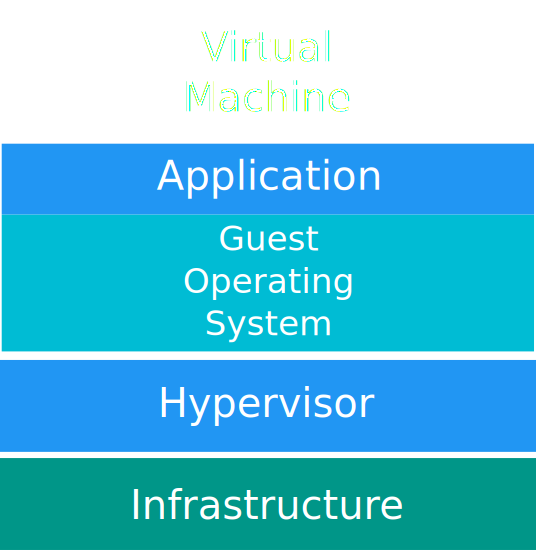
\includegraphics[scale=.45]{hypervisor_type1.pdf}

				Type 1 (\textit{e.g.} \texttt{xen} \cite{xen_contributors_xen_nodate})
			\end{column}
			\begin{column}{.5\textwidth}<2->
				\centering

				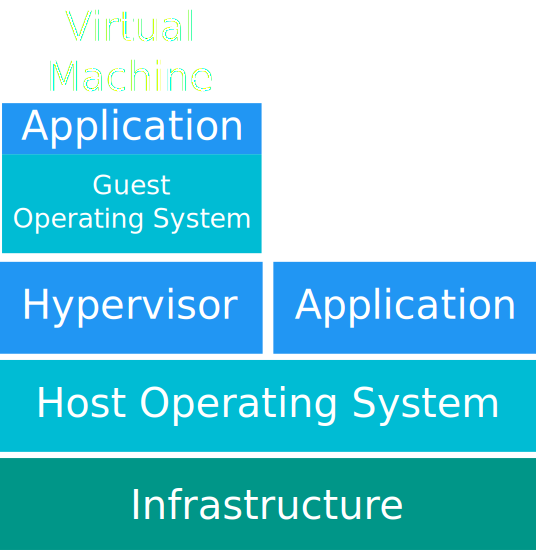
\includegraphics[scale=.45]{hypervisor_type2.pdf}

				Type 2 (\textit{e.g.} \texttt{virtualbox} \cite{vbox_contributors_virtualbox_nodate})
			\end{column}
		\end{columns}
	\end{frame}

	\begin{frame}
		\frametitle{The Quick EMUlator (\texttt{QEMU} \cite{qemu_contributors_qemu_nodate})}

		\begin{columns}
			\begin{column}{.5\textwidth}
				\texttt{QEMU}
				\begin{itemize}
					\item emulates the hardware,
					\item can run full system with \texttt{qemu-system-*}
					\item or single binary for other architecture with \texttt{qemu-user-*}
				\end{itemize}
			\end{column}
			\begin{column}{.5\textwidth}<2->
				\centering

				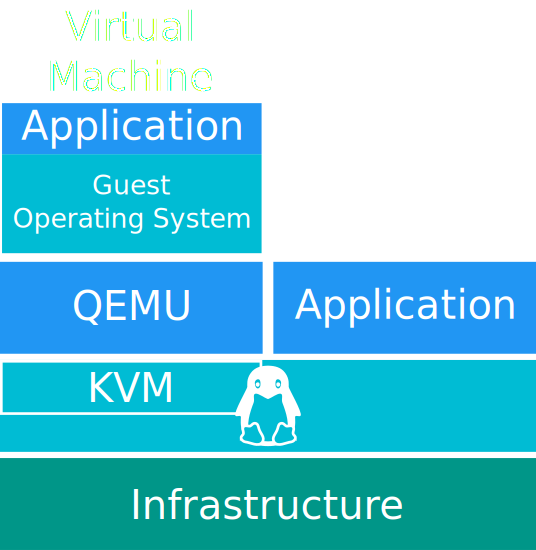
\includegraphics[scale=.45]{kvm.pdf}

				Speed up with KVM \cite{noauthor_introduction_nodate}!
			\end{column}
		\end{columns}
	\end{frame}

	\begin{frame}
		\frametitle{QEMU/KVM VM (simplified) boot process}

		\centering

		\includegraphics<1>{simplified_boot_process-fig1.pdf}%
		\includegraphics<2>{simplified_boot_process-fig2.pdf}%

		\onslide<2>{QEMU embeds BIOS, so it can jump directly on Linux!}
	\end{frame}

	\section{Conclusion}
	\begin{frame}
		\frametitle{Conclusion and demo}

		Conclusion:
		\begin{enumerate}
			\item[\cmark] Linux kernel development with \texttt{QEMU} is possible.
			\item[\cmark] It speeds up kernel development compared to previous method.
			\item[\xmark] But can only be used if you do not develop for specific hardware.
		\end{enumerate}

		\bigskip

		\onslide<2->{
			Demo time \cite{laniel_qemu_2018}!
		}
	\end{frame}

	\begin{frame}[allowframebreaks, noframenumbering]
		\frametitle{Bibliography}
		\setbeamertemplate{bibliography item}[text]

		\begin{scriptsize}
			\bibliographystyle{IEEEtran}
			\bibliography{beamer}
		\end{scriptsize}
	\end{frame}
\end{document}
